\documentclass[10pt]{article}
\usepackage{amsmath,amssymb,amsthm,amsfonts,hyperref,fancyhdr,graphicx,subfig,bbm,verbatim,float,microtype,multirow,array,titlesec}
\usepackage[export]{adjustbox}
\usepackage[dvipsnames]{xcolor}
\usepackage[left=2cm,right=2cm,top=2cm,bottom=2cm]{geometry}
\usepackage[none]{hyphenat}
\usepackage[justification=centering]{caption}
\graphicspath{{../figures/balanced/}}
\setlength{\parindent}{0cm}
\titleformat*{\section}{\Large\bfseries}
\titleformat*{\subsection}{\large\bfseries}

\newcommand{\R}{\mathbb{R}}
\newcommand{\1}{\mathbbm{1}}
\newcommand{\0}{\mathbf{0}}
\newcommand{\p}{\mathbb{P}}

\renewcommand{\baselinestretch}{1.2}
\newcolumntype{M}[1]{>{\raggedright}m{#1}}

\begin{document}
\begin{center}
\sc\Large Bootstrapping - noisy labels \\ {\small\today}
\end{center}
\vspace{-10pt}


\subsection*{Bootstraping the baseline 20\%\footnote{Balanced dataset with 20\% of positive samples}  (th=30) }
\subsubsection*{Update rules : relabelling the training set \label{score}}

(1) $\text{new decision score} =\dfrac12\bigg(\text{CNN score + previous score }\bigg)$, where CNN score = 100 $\hat{\mathbb P}(\text{label}=1)$\\
Update training set labels with a threshhold at $th^{(i+1)}=\frac{th^{(i)}+50}2$\\

\vspace{10pt}
(2: mean) $\text{new decision score} =mean(\text{CNN score , all previous scores })$\\
Update training set labels with a threshhold at $th=50$

\subsection*{Performance (1)}
\begin{figure}[H]
    \centering
    \subfloat[Training set]{\includegraphics[height=9cm]{strap_roc_train}}
    \subfloat[Test set]{\includegraphics[height=9cm]{strap_roc_test}}
\end{figure}
\begin{figure}[H]
    \centering
    \includegraphics[width=14cm]{strap_acc_loss}
    \caption{Accuracy \& losses - b5: baseline with original dataset (5\% of positive samples), b20: baseline with balanced dataset, strap i: i\textsuperscript{th} iteration of bootstrapping }
\end{figure}

\subsection*{Performance (2: mean)}
\begin{figure}[H]
    \centering
    \subfloat[Training set]{\includegraphics[height=9cm]{strap2_roc_train}}
    \subfloat[Test set]{\includegraphics[height=9cm]{strap2_roc_test}}
\end{figure}
\begin{figure}[H]
    \centering
    \includegraphics[width=14cm]{strap2_acc_loss}
    \caption{Accuracy \& losses}
\end{figure}

\subsubsection*{Labels update}
\begin{table}[H]
    \centering
    \begin{tabular}{|c|c|c|c|c|c|c|c|}
    \hline
           & baseline 20     &  strap 1      & strap 2    &   strap3    & strap 4  &  strap 5 &  strap 6\\
    \hline
    strap 1&    1039//3325   &               &            &             &          &          &          \\
    strap 2&    963//4659    &  368//1778    &            &             &          &          &          \\
    strap 3&     971//4811   &  441//1995    &  408//552  &             &          &          &          \\
    strap 4&     902//4960   &  426//2198    &  450//812  & 344//562    &          &          &          \\
    strap 5&     923//5014   &  445//2250    &  448//843  & 330//581    & 319//352 &          &          \\
    strap 6&    1055//4857   &  640//2156    &  768//874  & 708//670    & 520//264 & 594//305 &          \\
    strap 7&     950//5119   &  552//2435    &  660//1133 & 607//936    & 405//516 & 496//574 & 127//494 \\

    \hline
    \end{tabular}
    \caption{$|0\rightarrow 1|$//$|1\rightarrow 0|$}
\end{table}
\vspace{-5pt}
\subsubsection*{Labels update - mean}
\begin{table}[H]
    \centering
    \begin{tabular}{|c|c|c|c|c|c|c|}
    \hline
           & baseline 20     &  strap 1      & strap 2    &   strap3     &   strap4  & strap 5  \\
    \hline
    strap 1&    1039//3325   &               &            &              &           &          \\
    strap 2&     556//4983   &  78//2219     &            &              &           &          \\
    strap 3&     554//4857   &  89//2106     & 392//268   &              &           &          \\
    strap 4&     493//5016   &  63//2300     & 336//432   &   199//419   &           &          \\
    strap 5&     617//4933   &  122//2152    & 407//296   &   268//281   &  402//195 &          \\
    strap 6&     908//4827   &  434//2067    & 896//388   &   736//352   &  889//285 &  628//231\\
    \hline
    \end{tabular}
  %  \caption{$|0\rightarrow 1|$//$|1\rightarrow 0|$}
\end{table}
{\small We drop the initial score when computing the new score for the 5\textsuperscript{th} bootstrap iteartion and consider only the previous score for the 6\textsuperscript{th} iteration}

\subsubsection*{Confusion matrices}
q00$=\mathbb P(\text{true label}=0 |\text{predicted label} =0)$\\
q11$=\mathbb P(\text{true label}=1 |\text{predicted label} =1)$ \\
    % \[Q_{\text{full train}}=\begin{pmatrix}.9788&.0212\\.2935&.7065\end{pmatrix},
    % Q_{\text{balanced 20\%}}=\begin{pmatrix}.9811&.0189\\.2935&.7065\end{pmatrix},
    % Q_{\text{strap1}}=\begin{pmatrix}.9879&.0121\\.1625&.8375\end{pmatrix}\]
    % \[Q_{\text{strap2}}=\begin{pmatrix}.9837&.0163\\.1027&.8973\end{pmatrix},
    % Q_{\text{strap3}}=\begin{pmatrix}.9881&.0119\\.1007&.8993\end{pmatrix},
    % Q_{\text{strap4}}=\begin{pmatrix}.9867&.0133\\.634&.9366\end{pmatrix}\]
    % \[Q_{\text{strap5}}=\begin{pmatrix}.9867&.0133\\.0567&.9433\end{pmatrix}, 
    % Q_{\text{strap6}}=\begin{pmatrix}.9881&.0119\\.0759&.9241\end{pmatrix},
    % Q_{\text{strap7}}=\begin{pmatrix}.9868&.0132\\.0292&.9708\end{pmatrix}\]
Evaluated on a subset of the training set (606 negatives / 214 positives):
\begin{table}[H]
\centering
\begin{minipage}{.45\textwidth}
    \flushright
    \begin{tabular}{|c|c|c|}
    \hline
                   &   q00   &   q11\\
    \hline
    baseline 5\%   &  .9788   &  .7065  \\
    baseline 20\%  &  .9811   &  .7065  \\
    strap 1        &  .9879   &  .8375  \\
    strap 2        &  .9837   &  .8973  \\
    strap 3        &  .9881   &  .8993  \\
    strap 4        &  .9867   &  .9366  \\
    strap 5        &  .9867   &  .9433  \\
    strap 6        &  .9881   &  .9241  \\
    strap 7        &  .9868   &  .9708  \\
    \hline
    \end{tabular}
\end{minipage}
\begin{minipage}{.5\textwidth}
    \begin{tabular}{|c|c|c|}
    \hline
     Mean    &   q00    &   q11\\
    \hline
    && \\
    && \\
    && \\
    strap 2  &  .9794   &  .9209  \\
    strap 3  &  .9823   &  .9155  \\
    strap 4  &  .9809   &  .9281  \\
    strap 5  &  .9795   &  .9275  \\
    strap 6  &  .9866   &  .9110  \\
    &&\\
    \hline
    \end{tabular}
\end{minipage}
\end{table}
\subsubsection*{False positives \& false negatives in the training set}
\begin{table}[H]
    \begin{tabular}{|c|c|c||c|c|c|c|c|c|c|}
    \hline
            & baseline & baseline 20\% & strap 1 & strap 2 & strap 3  & strap 4 & strap 5  & strap 6   & strap 7\\
    \hline
    size    & 381942   & 79135         & ..      & ..      &  ..      & ..      &  ..      & ..        & ..     \\
    (1)\%   &  4.14\%  &   20\%        & 17.11\% & 15.33\% &  15.28\% & 14.87\% & 14.83\%  & 15.2\%    & 14.73\% \\
    FP      & 1461     &  1590         & 513     &   729   &   704    & 604     &  1176    &  264      &  403    \\
    FN      & 3919     &  4036         & 2198    &   670   &   1052   & 596     &   456    &  941      &  789   \\
    \hline
    \end{tabular}
    \vspace{10pt}
    \\
    \vspace{10pt}
    \textbf{Mean}:\\
    \begin{tabular}{|c|c|c||c|c|c|c|c|c|}
    \hline
            & baseline & baseline 20\% & strap 1 & strap 2         &  strap 3         &  strap 4    & strap 5    & strap 6\\
    \hline
    size    & 381942   & 79135         & ..      & ..              &                  &             &            & \\
    (1)\%   &  4.14\%  &   20\%        & 17.11\% &    14.41\%      &   14.56\%        &    14.28\%  &  14.55\%   & 15.05\%\\
    FP      & 1461     &  1590         & 513     &     492         &     540          &     244     &   839      & 361    \\
    FN      & 3919     &  4036         & 2198    &     618         &     783          &    1179     &   274      & 1169 \\
    \hline
    \end{tabular}
\end{table}
\newpage
\subsubsection*{(Mis)classified samples from the training set}
\textbf{The baseline:}
\begin{figure}[H]
    \centering
    \subfloat[False negatives - 85\% mislabelled]{
    \includegraphics[width=9cm,cfbox=gray 1pt 1pt]{FNFP/gray_FN_b}}
    \subfloat[False positives - 46\% mislabelled]{
    \includegraphics[width=9cm,cfbox=gray 1pt 1pt]{FNFP/gray_FP_b}}
    \caption{Annotation : CNN score / Initial classifier score}
\end{figure}
\textbf{1st iteration:}
\begin{figure}[H]
    \centering
    \subfloat[False negatives - 78\% mislabelled]{
    \includegraphics[width=9cm,cfbox=gray 1pt 1pt]{FNFP/gray_FN_s1}}
    \subfloat[False positives - 42\% mislabelled]{
    \includegraphics[width=9cm,cfbox=gray 1pt 1pt]{FNFP/gray_FP_s1}}
    \caption{Strap 1: annotation = CNN score//scores history}
\end{figure}

% \textbf{2nd iteration:}
% \begin{figure}[H]
%     \centering
%     \subfloat[False negatives - 71\% mislabelled]{
%     \includegraphics[width=9cm,cfbox=gray 1pt 1pt]{FNFP/gray_FN_s2}}
%     \subfloat[False positives - 51\% mislabelled]{
%     \includegraphics[width=9cm,cfbox=gray 1pt 1pt]{FNFP/gray_FP_s2}}
%     \caption{Strap 2: annotation = CNN score//scores history}
% \end{figure}

% \textbf{3rd iteration:}
% \begin{figure}[H]
%     \centering
%     \subfloat[False negatives - 49\% mislabelled]{
%     \includegraphics[width=9cm,cfbox=gray 1pt 1pt]{FNFP/gray_FN_s3}}
%     \subfloat[False positives - 44\% mislabelled]{
%     \includegraphics[width=9cm,cfbox=gray 1pt 1pt]{FNFP/gray_FP_s3}}
%     \caption{Strap 3: annotation = CNN score//scores history}
% \end{figure}
% \newpage
% \textbf{4th iteration:}
% \begin{figure}[H]
%     \centering
%     \subfloat[False negatives - 49\% mislabelled]{
%     \includegraphics[width=9cm,cfbox=gray 1pt 1pt]{FNFP/gray_FN_s4}}
%     \subfloat[False positives - 49\% mislabelled]{
%     \includegraphics[width=9cm,cfbox=gray 1pt 1pt]{FNFP/gray_FP_s4}}
%     \caption{Strap 4: annotation = CNN score//scores history}
% \end{figure}
% \textbf{5th iteration:}
% \begin{figure}[H]
%     \centering
%     \subfloat[False negatives - 41\% mislabelled]{
%     \includegraphics[width=9cm,cfbox=gray 1pt 1pt]{FNFP/gray_FN_s5}}
%     \subfloat[False positives - 24\% mislabelled]{
%     \includegraphics[width=9cm,cfbox=gray 1pt 1pt]{FNFP/gray_FP_s5}}
%     \caption{Strap 5: annotation = CNN score//scores history}
% \end{figure}
% \newpage
% \textbf{6th iteration:}
% \begin{figure}[H]
%     \centering
%     \subfloat[False negatives - 37\% mislabelled]{
%     \includegraphics[width=9cm,cfbox=gray 1pt 1pt]{FNFP/gray_FN_s6}}
%     \subfloat[False positives - 27\% mislabelled]{
%     \includegraphics[width=9cm,cfbox=gray 1pt 1pt]{FNFP/gray_FP_s6}}
%     \caption{Strap 6: annotation = CNN score//scores history}
% \end{figure}
\newpage
\textbf{7th iteration:}
\begin{figure}[H]
    \centering
    \subfloat[False negatives - 39\% mislabelled]{
    \includegraphics[width=9cm,cfbox=gray 1pt 1pt]{FNFP/gray_FN_s7}}
    \subfloat[False positives - 55\% mislabelled]{
    \includegraphics[width=9cm,cfbox=gray 1pt 1pt]{FNFP/gray_FP_s7}}
    \caption{Strap 7: annotation = CNN score//scores history}
\end{figure}
% \newpage
% \textbf{2nd -mean iteration:}
% \begin{figure}[H]
%     \centering
%     \subfloat[False negatives - 53\% mislabelled]{
%     \includegraphics[width=9cm,cfbox=gray 1pt 1pt]{FNFP/gray_FN_bs2}}
%     \subfloat[False positives - 65\% mislabelled]{
%     \includegraphics[width=9cm,cfbox=gray 1pt 1pt]{FNFP/gray_FP_bs2}}
%     \caption{Strap 2 -mean: annotation = CNN score//scores history}
% \end{figure}
% \textbf{3rd -mean iteration:}
% \begin{figure}[H]
%     \centering
%     \subfloat[False negatives - 50\% mislabelled]{
%     \includegraphics[width=9cm,cfbox=gray 1pt 1pt]{FNFP/gray_FN_bs3}}
%     \subfloat[False positives - 66\% mislabelled]{
%     \includegraphics[width=9cm,cfbox=gray 1pt 1pt]{FNFP/gray_FP_bs3}}
%     \caption{Strap 3 -mean: annotation = CNN score//scores history}
% \end{figure}
% \newpage
% \textbf{4th -mean iteration:}
% \begin{figure}[H]
%     \centering
%     \subfloat[False negatives - 31\% mislabelled]{
%     \includegraphics[width=9cm,cfbox=gray 1pt 1pt]{FNFP/gray_FN_bs4}}
%     \subfloat[False positives - 73\% mislabelled]{
%     \includegraphics[width=9cm,cfbox=gray 1pt 1pt]{FNFP/gray_FP_bs4}}
%     \caption{Strap 4 -mean: annotation = CNN score//scores history}
% \end{figure}

% \textbf{5th -mean iteration:}
% \begin{figure}[H]
%     \centering
%     \subfloat[False negatives - 62\% mislabelled]{
%     \includegraphics[width=9cm,cfbox=gray 1pt 1pt]{FNFP/gray_FN_bs5}}
%     \subfloat[False positives - 53\% mislabelled]{
%     \includegraphics[width=9cm,cfbox=gray 1pt 1pt]{FNFP/gray_FP_bs5}}
%     \caption{Strap 5 -mean: annotation = CNN score//scores history}
% \end{figure}

% \newpage

\textbf{6th -mean iteration:}
\begin{figure}[H]
    \centering
    \subfloat[False negatives - 40\% mislabelled]{
    \includegraphics[width=9cm,cfbox=gray 1pt 1pt]{FNFP/gray_FN_bs6}}
    \subfloat[False positives - 43\% mislabelled]{
    \includegraphics[width=9cm,cfbox=gray 1pt 1pt]{FNFP/gray_FP_bs6}}
    \caption{Strap 5 -mean: annotation = CNN score//scores history}
\end{figure}
\end{document}

%------------------------------------------------------------------------------ Deleted
\subsection*{Changing the baseline}
(1) Reduce the base learning rate from $10^{-2}$ to $10^{-4}$\\
The losses and accuracy remains jumpy and the ROC curve is worse than the baseline 20\%.\\
(2) Remove the dropout after the fully connected layers.\\
(3) Change the solver from stochastic to adaptive gradient descent.\\

\begin{figure}[H]
    \centering
    \includegraphics[width=12cm]{acc_loss}
    \caption{}
\end{figure}

\begin{figure}[H]
    \centering
    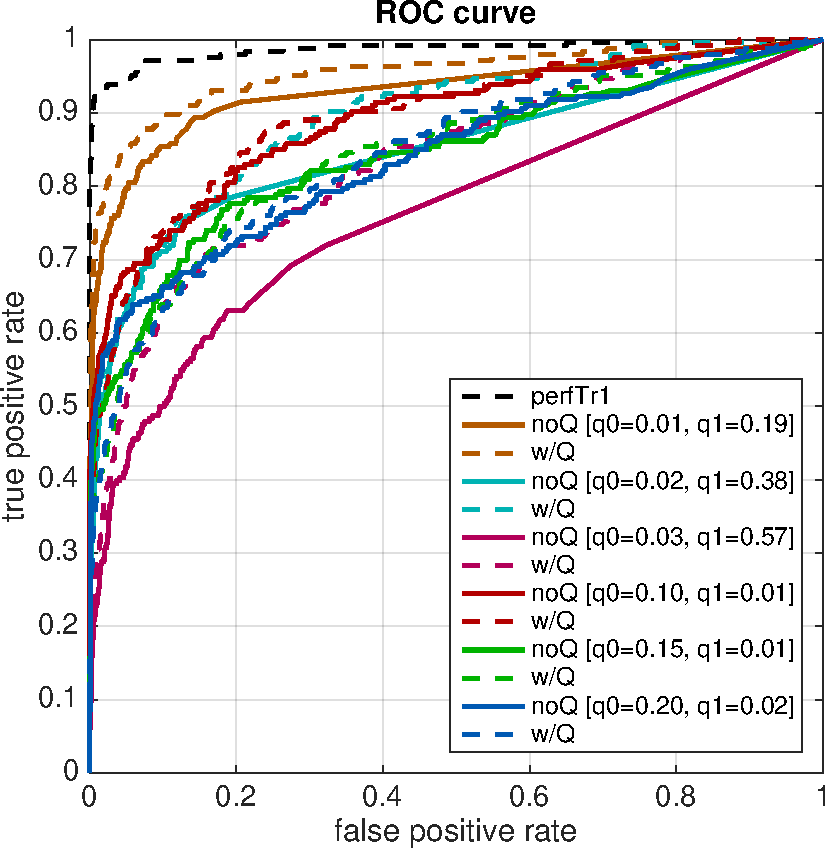
\includegraphics[width=8cm]{roc}
    \caption{}
\end{figure}



plot(bs3.data(:,1),bs3.data(:,4),'color','r')
\section*{Bootstraping the baseline 5\% for th=30 }
\subsection*{Confusion matrices}
\[Q_{\text{strap 1}}=\begin{pmatrix}.9785&.0215\\.1467&.8533\end{pmatrix}\]

% My roc curves 1-tnr, tpr i.e FPR ,TPR
%       TP(S) = num. of samples that are correctly classified as positive,
%       TN(S) = num. of samples that are correctly classified as negative,
%       FP(S) = num. of samples that are incorrectly classified as positive,
%       FN(S) = num. of samples that are incorrectly classified as negative.
%
%     Consider also the rates:
%
%       TPR = TP(S) / P,      FNR = FN(S) / P,
%       TNR = TN(S) / N,      FPR = FP(S) / N,
%
%     and notice that, by definition,
%
%       P = TP(S) + FN(S) ,    N = TN(S) + FP(S),
%       1 = TPR(S) + FNR(S),   1 = TNR(S) + FPR(S).